% add --shell-escape to pdflatex arguments.
% add following key to have keyboard shortcuts
%{
%    "key": "shift+b",
%    "command": "commandId",
%    "when": "editorTextFocus"
%},
%{
%"key": "shift+B",
%"command": "editor.action.insertSnippet",
%"when": "editorLangId == latex && editorTextFocus",
%"args": {
%    "snippet": "\\textbf{${TM_SELECTED_TEXT}$0}"
%}
%}

\documentclass[14pt]{extarticle}
\usepackage[left=2cm , right = 2cm, top=2cm]{geometry}
\usepackage{helvet}
\usepackage{parskip}
\usepackage{amsmath}
\usepackage{amssymb}
\usepackage{graphicx}
\usepackage[spanish]{babel}
\usepackage[dvipsnames]{xcolor}
\usepackage{tcolorbox} % above of the svg package
\usepackage{svg} 
\usepackage{hyperref}
\usepackage{minted}
\renewcommand{\sfdefault}{lmss}  % este activa la letra lmss
\renewcommand{\familydefault}{\sfdefault} % este activa la letra lmss
\sffamily % este activa la letra lmss
%\hyperlink{page.2}{Go to page 2}
%\newpage
%text on page 2
%\begin{figure}[htbp]
%  \centering
%  \includesvg{plot.svg}
%  \caption{svg image}
%\end{figure}

%\begin{minted}{csharp}
%    // single comment
%    \end{minted}

% f(n) = \begin{cases}
%    n/2  & n \text{ is even} \\
%    3n+1 & n \text{ is odd}
%  \end{cases}

%\begin{align}
%    \frac{d}{dx} \ln x &= \lim_{h\to 0} \frac{\ln(x+h) - \ln x}{h} \\
%    &= \ln e^{1/x} &&\text{How this follows is left as an exercise.}\\
%    &= \frac{1}{x} &&\text{Using the definition of ln as inverse function}
%   \end{align}


\begin{document}

\section{Repositorio}

% add an hyperlink
\href{https://github.com/BritoAlv/SRI-hybrid-techniques-in-recommendation-systems}{SRI-hybrid-techniques-in-recommendation-systems}


\section{Autores}
\begin{enumerate}
    \item David Lezcano Becerra C-312 \href{https://github.com/david-dlb}{@david-dlb}
    \item Javier Lima García C-312 \href{@limaJavier}{https://github.com/limaJavier}
    \item Álvaro Luis González Brito C-312 \href{@BritoAlv}{https://github.com/BritoAlv}
\end{enumerate}


\section{Recomendación híbrida}

Como su nombre indica, la recomendación híbrida pretende tomar lo mejor de ambos mundos (basado en contenido y colaborativo) para amplificar el poder de los sistemas de recomendación. Pueden utilizarlos de manera separada para después combinar los resultados ponderadamente o bajo selección, o integrarlos directamente en un solo modelo.

Netflix es un buen ejemplo de esto, esta plataforma ofrece recomendaciones comparando los hábitos de búsqueda y visualizaciones de usuarios similares, así como, ofreciendo películas que comparten características similares con aquellas que el usuario ha tenido en alta estima.

\section{Antecedentes}

Elaine Rich creó el primer Sistema de Recomendación en 1979, llamado \textbf{Grundy}. Buscaba una forma de recomendar a usuarios libros que les pudieran gustar. Su idea fue crear un sistema que realizara preguntas específicas y las clasificara en clases de preferencias o \textbf{estereotipos}, en dependencia de sus respuestas. Basado en esta pertenencia a un cierto estereotipo, los usuarios recibirían recomendaciones de libros.

Otro de los primeros Sistemas de Recomendación, es el llamado \textbf{librero digital} (digital bookshelf), el cual fue descrito en un reporte técnico en 1990 por Jussi Karlgren en la Universidad de Columbia, e implementado a escala y continuado mediante reportes técnicos y publicaciones desde 1994 en adelante por Jussi Karlgren, en ese entonces en el SICS, en conjunto con el grupo investigativo dirigido por Pattie Maes del MIT, Will Hill de Bellcore y Paul Resnick, también del MIT. Este trabajo, junto con GroupLens, fue premiado en 2010 por la ACM Software Systems Award.

\section{Descripción del Tema}

Hoy en día son numerosas las aplicaciones en las que confluyen usuarios para consumir, comprar, o vender un conjunto de productos, servicios, artículos o propiedades. Dada la infinidad de opciones que poseen los usuarios, se dificulta no solo la búsqueda de lo deseado, sino que incluso estos desconocen o son incapaces de encontrar aquello que realmente estaban buscando y dejan pasar opciones óptimas ajustadas a sus necesidades, preferencias o recursos.

Este problema, acrecentado por la magnitud de datos de la actualidad, ha sido objetivo de muchas investigaciones y ha dado a luz a los \textbf{Sistemas de Recomendaciones}. Estos sistemas son capaces de acercar aquellos productos (recursos, artículos, etc) que satisfacen las preferencias y necesidades particulares de cada usuario; de ahí que plataformas como Netflix, Amazon, YouTube o Spotify los utilicen y hayan contribuido profundamente al desarrollo de estos.

Existen dos tipos fundamentales de Sistemas de Recomendación: el \textbf{filtrado por contenido} (content-base filtering) y el \textbf{filtrado por colaboración} (collaborative filtering).

\textbf{Nota}: Por motivos de simplicidad se decide utilizar `productos` para referirse a todo lo que los Sistemas de Recomendación puedan ofrecer, así como `consumir` para todas las acciones que los usuarios puedan hacer con estos productos.

\subsection{Filtrado por contenido}

\begin{figure}[H]
    \centering
    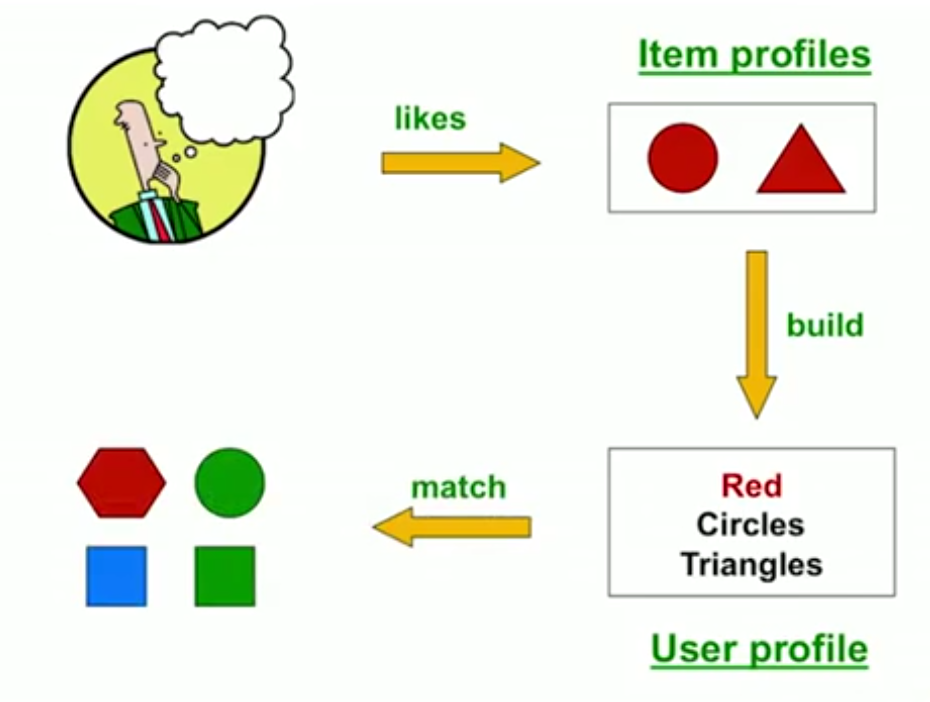
\includegraphics[width=\textwidth]{./images/content-bases_filtering.png}
    \caption{Filtrado por contenido}
    \label{Filtrado por contenido}
\end{figure}


La idea fundamental del \textbf{filtrado por contenido} radica en: \textbf{recomendar a un usuario productos similares a aquellos que el usuario previamente ha consumido}

De esta idea se deriva la siguiente cuestión: ¿cómo encontrar los artículos similares?

Numerosas estrategias han sido diseñadas para responder a esta pregunta y dentro de estas resalta la \textbf{construcción de perfiles}. Esta, se basa en la creación de perfiles para los productos y para los usuarios, fundamentalmente, creando una representación vectorial de estos:

\begin{enumerate}
    \item Los productos son vectorizados teniendo en cuenta el contexto, metadatos y requerimientos (vectores reales o vectores booleanos).
    \item Los vectores asociados a usuarios pueden obtenerse por numerosas vías, desde un simple promedio de los vectores asociados a productos consumidos, a un promedio ponderado o incluso utilizando técnicas basadas en Machine Learning.
\end{enumerate}

Una vez llevada a cabo la vectorización, puede usarse directamente la \textbf{similitud del coseno} para encontrar aquellos perfiles de productos más similares al perfil del usuario seleccionado.

\subsection{Filtrado colaborativo}

\begin{figure}[H]
    \centering
    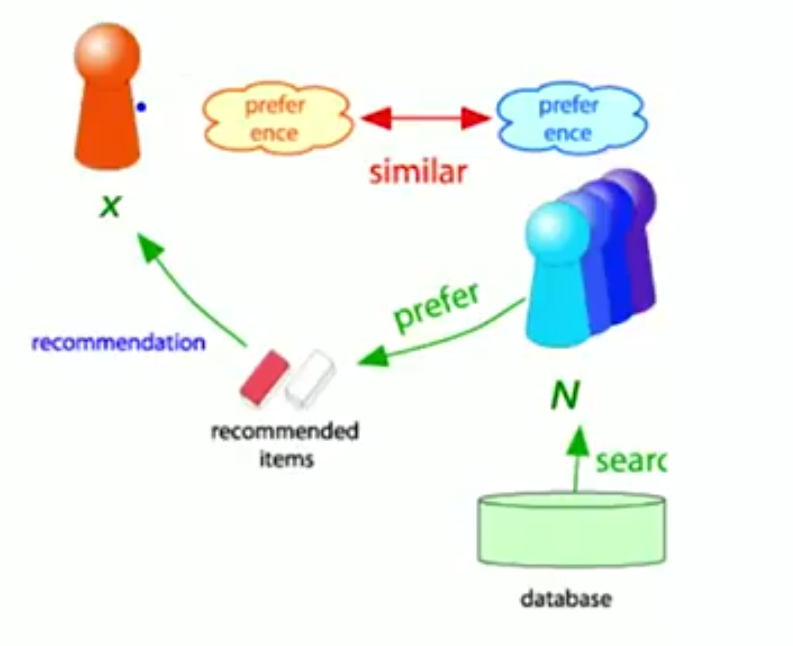
\includegraphics[width=\textwidth]{./images/collaborative_filtering.png}
    \caption{Collaborative Filtering}
    \label{Collaborative Filtering}
\end{figure}

El \textbf{filtrado colaborativo} posee dos vertientes distintas, y teóricamente equivalentes llamadas:

    \begin{enumerate}
        \item Usuario-Usuario (user to user): \textbf{Recomendar a un usuario aquellos productos que han consumido usuarios similares a él/ella}
        \item Producto-Producto (item to item): \textbf{Recomendar un producto a un usuario si productos similares a este han sido consumidos previamente por dicho usuario}
    \end{enumerate}

Como en el método anterior se nos presenta nuevamente el problema de la similaridad, sin embargo, a diferencia de este, en el filtrado colaborativo se cuenta con la \textbf{matriz de similaridad}, cuyas coordenadas, por ejemplo, $(i, j)$ contienen cuánto ha estimado (rated en inglés) el usuario $i$ al producto $j$. 

Con esta matriz y utilizando, generalmente, la similitud \textbf{centrada del coseno} (centered cosine similarity) conocida también como \textbf{Correlación de Pearson} (Pearson Correlation), podemos predecir cuánto estimará un usuario un determinado producto, de la siguiente manera:

\textbf{Usuario-Usuario:}

Para un producto $i$ y usuario $x$, donde $N$ es el conjunto de los $k$ usuarios más similares a $x$ que han consumido el producto $i$, la predicción es la siguiente:

$$r_{xi} = \frac{\sum_{y \in \mathbb{N}} s_{xy} r_{yi}}{\sum_{y \in \mathbb{N}} s_{xy}}$$


\textbf{Producto-Producto}

Para un producto $i$ y un usuario $x$, donde $N$ es el conjunto de los $k$ productos más similares a $i$ que han sido consumidos por $x$, la predicción es la siguiente:

$$r_{xi} = \frac{\sum_{j \in \mathbb{N} (i; x)} s_{ij} r_{xj}}{\sum_{j \in \mathbb{N} (i;x)} s_{ij}}$$


Para ambos casos, $s$ es la similitud (en el primero entre usuarios y en el segundo entre productos) y $r$ cuánto ha estimado al producto.

Como se mencionó previamente, ambas estrategias del filtrado colaborativo son teóricamente equivalentes (incluso podrían considerarse duales), sin embargo, en la práctica \textbf{Producto-Producto} vence a \textbf{Usuario-Usuario}, y esto, debido, a que los productos son más "sencillos" que los usuarios en el sentido de que es más fácil clasificarlos (géneros en la música, estilos en pintura, etc.), mientras que los usuarios son más impredecibles, lo que lleva a que el criterio de similitud entre productos aporte una mayor relevancia que entre usuarios.

\section{Datos Utilizados}

La información utilizada para el proyecto se encuentra almacenada en una base de datos (específicamente utilizamos SQLite como SGBD), que contiene como tablas principales: \textbf{Books}, \textbf{Users} y \textbf{UserBooks} (presenta los datos obtenidos de una interacción usuario libro, como: rating, comentarios, cantidad de shares y ratio de lectura)

La información presente en esta base de datos fue obtenida de dos formas, utilizando el script "data collector":

\begin{enumerate}
    \item Para los metadatos sobre los libros (tabla \textbf{Books}) fue utilizada la \href{https://gutendex.com/}{API Gutendex}, que provee los metadatos de los libros almacenados por el Proyecto Gutenberg.
    \item Para los usuarios (tabla \textbf{Users}) y las interacciones usuario-libro (tabla \textbf{UserBooks}), se simuló el comportamiento de estos con respecto a un conjunto de libros.
\end{enumerate}

\subsection{Extracción de los libros}

La extracción de los metadatos asociados a libros fue bastante directa a través de  \href{https://gutendex.com/}{Gutendex}. La única transformación realizada se produjo durante la extracción de los géneros; y es que, dada la multitud de géneros existentes, predefinimos un conjunto de estos (tabla \textbf{Genres}), y según la similitud de estos con la sección `subject` de los datos de la API, añadimos los géneros a cada libro.

\subsection{Generación de usuarios e interacciones}

Para generar usuarios e interacciones con libros lo más cercano a la realidad, se decidió utilizar la siguiente estrategia:

Dado los \textbf{k} libros más populares y los \textbf{p} autores más populares (la API brinda la información de cuántas veces un libro ha sido descargado), se generó un usuario que va a presentar tres características distintas, generadas aleatoriamente:

\begin{enumerate}
    \item Época preferida (antigua, moderna o contemporánea)
    \item Autores preferidos (de los autores más populares)
    \item Géneros preferidos
\end{enumerate}

Con este perfil de usuario se procedió a escoger de $1$ a $300$ libros (de los más populares) con los que el usuario potencialmente interactuará. Por cada libro validamos lo siguiente:

\begin{enumerate}
    \item Si el libro pertenece a un género que le gusta al usuario, o su autor es uno de los preferidos del usuario, o pertenece a la época favorita del usuario, entonces tendrá una interacción "positiva" (más adelante se explicará en qué consiste)
    \item Si no se cumple ninguna condición anterior entonces tendrá una interacción "negativa"
\end{enumerate}

\subsection{Interacciones:}

Una \textbf{interacción positiva} colocará de manera aleatoria valores considerados positivos para la interacción, de manera \textbf{análoga} se produce para una \textbf{interacción negativa}. A forma de ejemplo, mostramos nuestra implementación:

\begin{minted}{python3}
    def _positive_user_book(self, user_id : int, book_id : int):
        shared = random.randint(3, 20)
        read_ratio = random.randint(50, 100) / 100
        rating = random.randint(3, 5)
        comment = random.choice([
            'It is a really good book. I would read it again',
            'Just love it',
            'I would recommend this book to anyone. It is a hidden diamond'
        ])

        user_book = UserBook(user_id, book_id)
        user_book.shared = shared
        user_book.readRatio = read_ratio
        user_book.rating = rating
        user_book.comment = comment
        return user_book

def _negative_user_book(self, user_id : int, book_id : int):
    shared = random.randint(0, 2)
    read_ratio = random.randint(0, 50) / 100
    rating = random.randint(0, 2)
    comment = random.choice([
        "Simply don't like the book",
        "It's awful",
        "Terrible book! (in the bad sense)"
    ])

    user_book = UserBook(user_id, book_id)
    user_book.shared = shared
    user_book.readRatio = read_ratio
    user_book.rating = rating
    user_book.comment = comment
    return user_book    
\end{minted}

\subsection{Análisis Estadístico }

Fue realizado un análisis estadístico sobre los datos generados para comprobar el comportamiento de anomalías que pudieran afectar la validez de nuestro sistema de recomendación. Para esto se tomó como referencia la cantidad de cada uno de los ratings ("overall" en este caso) por usuario y por libros.

\begin{figure}[H]
    \centering
    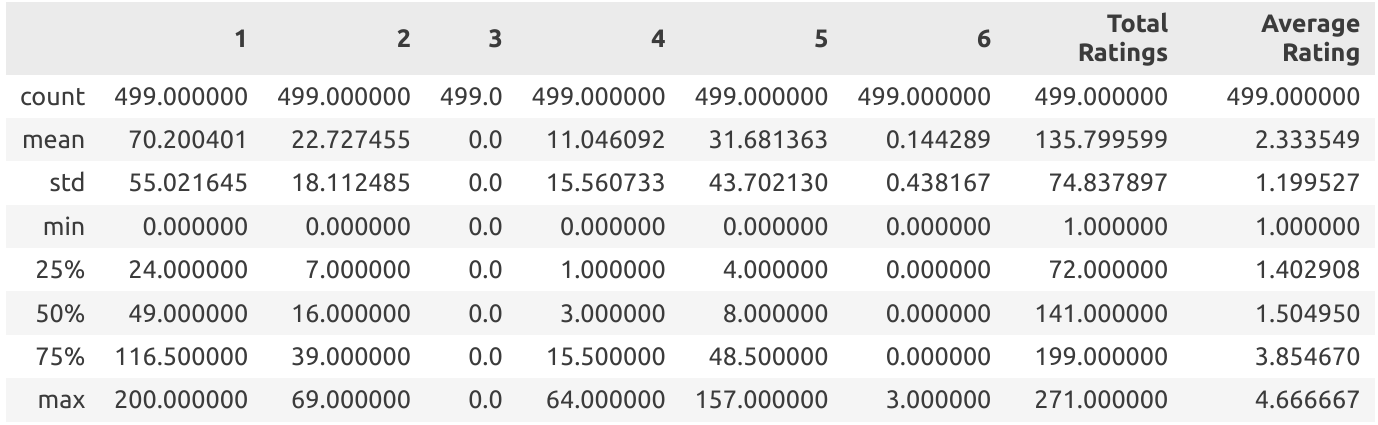
\includegraphics[width=\textwidth]{./images/general_stats.png}
    \caption{Collaborative Filtering}
    \label{Collaborative Filtering}
\end{figure}

Como podemos apreciar por una descripción global de los datos seleccionados, existe una tendencia hacia los ratings negativos, así como una nula y casi nula existencia de ratings de 3 y 6, respectivamente. Dado que es poco común que esto se produzca con datos reales, fue realizado un análisis más profundo utilizando el \textbf{z-score}. Los resultados obtenidos fueron los siguientes:

\begin{enumerate}
    \item $3\%$ de los datos asociados a usuarios presentan anomalías
    \item $0.03\%$ de los datos asociados a libros presentan anomalías
\end{enumerate}

Dada el bajo porcentaje de anomalías encontradas y el contexto del proyecto (no se trabaja con información financiera o médica de alto riesgo, por ejemplo), se decidió que los datos son viables para la prueba del sistema.

\section{Implementación}

Para recomendar una lista de libros a un usuario, no necesariamente registrado en nuestra aplicación, se usa un enfoque híbrido conocido por \textbf{Item-based Clustering Hybrid Method}, este combina \textbf{Content-Based and Collaborative Filters}, el resultado final de este algoritmo es una matriz de similitud $M[i][j]$ que representa la similitud que es determinada entre los libros $i, j$. Con esta matriz calculada es posible predecir un rating entre el usuario $u$ y el libro $b$, la salida de la aplicación serían los mejores $N$ ratings.   

El sistema recomendador, después de haber calculado la matriz de similitud $M$ puede hacer recomendaciones a usuarios, por lo que se distinguen dos estados en los que se puede encontrar este:

\begin{enumerate}
    \item a partir de información nueva sobre los usuarios o nuevos items calcular nuevamente esta matriz $M$.
    \item realizar recomendaciones a los usuarios ( registrados o no ).
\end{enumerate}

Para que nuestra aplicación se mantenga interactiva, cada cierto tiempo recalculamos esta matriz en segundo plano, y cuando se haya terminado este proceso, concurrentemente actualizamos la información, para que a partir de este momento se pueda usar la nueva información en la recomendación.


\subsection{Como Predecir Rating}  

Con la matriz de similitud $M$ se usa la siguiente fórmula para predecir el rating $r$ de un usuario $u$ a el libro $b$ :

$$r[u][b] = P_b + \frac{\sum_{i = 1}^n M[i][b]*(R[u][i] - P_i)}{\sum_{i = 1}^n | M[i][b] | }$$

Donde $n$ representa la cantidad de libros con los que el usuario $u$ ha interactuado y están en nuestra base de datos, $R[u][b]$ representa el rating de el usuario $u$ a el libro $b$ y $P_b$ representa el promedio de los ratings que ha recibido el libro $b$.

Los dos sumandos de la fórmula anterior son interpretados como:

\begin{enumerate}
    \item Notar que si el usuario no ha interactuado con ningún libro el sistema usaría solamente  los promedios de los ratings de los libros existentes ( el primer sumando ), lo que permite hacer recomendaciones a los usuarios sin tener conocimiento de ellos.
    \item Con respecto a la segunda fórmula, notar que el segundo factor de cada sumando representa una proporción con respecto a el denominador, o sea, representa un promedio ponderado. Si estos pesos fueran todos iguales a 1, fuera un promedio. En general la fórmula representa la desviación de los ratings obtenidos de el usuario con respecto a la media de ratings obtenidos de usuarios a ese libro, la idea de la ponderación es que los libros más similares a el libro $b$ que se intenta predecir obtengan más peso con respecto a los menos similares. 
\end{enumerate}

La complejidad de realizar este método sería $O(n)$, pero este es calculado por cada libro que hay en nuestra base de datos, asumiendo que hayan $m$ libros esta sería $O(n * m)$, por esta razón tenemos alrededor de $2000$ libros en nuestra base de datos, cifra que permite realizar la recomendación lo suficientemente rápido.

Dada la explicación anterior quedaría por analizar como es calculada la matriz $M$ de similitud:

Esta matriz es obtenida a través de la combinación linear de otras dos matrices, análogamente de similitud ($A[i][j]$ representa la similitud entre los libros $i, j$), que son halladas a partir de la información que posee el sistema:

\subsection{Matrices de Similitud}

Se describe como son obtenidas las dos matrices y posteriormente como son combinadas para obtener la matriz $M$:

\textbf{Matriz $1$:}

Sobre un usuario, en nuestra base de datos , contamos con alguna interacción con ciertos libros, usamos esta información para calcular un \textbf{rating} para cada libro con el que interactúa el usuario descrito como un número entre $[1,5]$. Hay varias formas de hallar este rating, describimos en otra sección el método usado. 

El resultado de el proceso anterior es conocido como \textbf{item-rating matrix}, nuestro objetivo es obtener una matriz de similitud a partir de esta \textbf{item-rating matrix}. Para hacerlo se usa el \textbf{Pearson Correlation Algorithm}, en particular la siguiente fórmula:

$$A[k][l] = \frac{ \sum_{u = 1}^m (R_{u,k} - R_k)*(R_{u,l} - R_l) }{ \sqrt{\sum_{u = 1}^m (R_{u,k} - R_k)^2} * \sqrt{\sum_{u = 1}^m (R_{u,l} - R_l)^2} }$$

Donde $k, l$ son dos libros en nuestra base de datos, $m$ es la cantidad de usuarios que interactuaron con ambos libros $k, l$. $R_k,R_l$ son los promedios de los rating recibidos por los libros $k, l$ y $R_{u,k}, R_{u,l}$ son los ratings de los libros $k, l$ dados por el usuario $u$. 

Por cada usuario que interactuó con ambos libros $k,l$ se obtiene un par $(x_1, y_1)$, en nuestro caso representan el rating obtenido, el coeficiente de Pearson mide la correlación linear entre dos samples $(x_1, x_2, ..., x_l)$, $(y_1, y_2, ..., y_l)$, este coeficiente es un número entre $-1$ y $1$, $1$ indicando que los puntos están alineados con pendiente positiva, $-1$, con pendiente negativa, $0$ es que no existe relación linear entre ellos, si están alineados con pendiente negativa es interpretado como que son contrarios, o no concuerdan.

\textbf{Matriz $2$:}

La matriz anterior usa información obtenida de la interacción usuario-libro, para esta matriz solamente es requerida información de los libros, es posible establecer una medida de similitud entre los libros, esto no es más que una función que toma como argumentos dos libros y devuelve un valor entre $0, 1$ como una medida de que tan similares son. 

Esta ha de cumplir ser reflexiva y simétrica. Hay varias formas de establecer esta similitud, en otra sección explicamos cual medida usamos. Asumiendo una función de similitud $f$, es posible ejecutar un algoritmo de $K-means$ para agrupar a los libros:

Este asigna inicialmente al azar $k$ grupos, representados cada uno por un libro.

En base a la similitud se calcula a cual grupo debe pertenecer cada libro, una vez realizado esto, es posible cambiar a el representante de cada grupo por otro libro en el grupo, que se encuentre más al \textbf{centro} con respecto a los libros en su grupo, teniendo en cuenta esto, el algoritmo es de punto fijo hasta que se logren centros de cada grupo \textbf{estables}. ( no cambiarían en una próxima iteración). 

Para cambiar a el representante de el grupo,  hay varias formas, en nuestro caso , por cada elemento de el grupo  hallamos su similitud con los restantes y multiplicamos esos valores, se mantiene como un número entre $[0, 1]$, escogemos como nuevo representante el que maximice ese valor.

Una vez que tenemos el \textbf{grouping} realizado se crea una matriz $T$ donde las filas son libros, y las columnas son los representantes de los grupos, en las casillas estaría la similitud entre el libro \textbf{fila} y el representante \textbf{columna} , esto puede ser visto como la \textbf{membership} de cada elemento a un conjunto, en términos de \textbf{fuzzy logic}.

Finalmente a partir de esta matriz $T$ se calcula la matriz de similitud, notar que la matriz de similitud es indexada con dos libros cualesquiera, mientras que esta $T$ es entre un libro y un libro representante de algún grupo.

Para hallar la matriz de similitud es usada una variación de la similitud de coseno, la idea es que las filas de la matriz ( libros ) representan un vector, y sus valores son los que están a lo largo de la fila, o sea, cada componente es uno de los grupos. La razón de la variación de la similitud de coseno es una cuestión de escalas: si un usuario siempre marca con $5$ su mejor película, $1$ una mala película a su juicio, mientras que otro, por costumbre, nunca marca con $5$ ni siquiera a su película preferida, sino con 4, y análogamente con $2$ a una película mala, ocurre una diferencia de escalas que no es manejada correctamente por la similitud de coseno estándar. La fórmula sería : 

$$A[k][l] = \frac{ \sum_{u = 1}^m (R_{k, u} - R_u)*(R_{l, u} - R_u) }{ \sqrt{\sum_{u = 1}^m (R_{k, u} - R_u)^2} * \sqrt{\sum_{u = 1}^m (R_{l, u} - R_u)^2} }$$

Donde $k, l$ son dos libros, $m$ es la cantidad de clusters, $R_{k,u}, R_{l,u}$ representa la similitud entre el libro $k$ y el representante del cluster $u$, análogamente $R_{l, u}$, $R_u$ es el promedio de las similitud respecto a el libro representante del cluster $u$, o ( sea el promedio de los valores en esa columna).

\subsection{Combinación}

Una vez calculadas las dos matrices $A_1, A_2$ entonces:

$$M = c * A_1 + (1-c) * A_2$$

La cantidad de clusters, y el coeficiente en la combinación linear son parámetros que deben estimarse de forma que minimicen alguna métrica como \textbf{Mean Absolute Error}.

\subsection{Complejidad}

La complejidad de todos estos pasos es al menos cuadrática : 

\begin{enumerate}
    \item el algoritmo de $K-Means$ divide a los libros en grupos, pero dentro de un  grupo es hallada la similitud entre cada par de libros, esto es $O(it * l^2)$ donde $it$ es la cantidad de iteraciones que hace el algoritmo, y $l$ es la cantidad de libros.

    \item el algoritmo para calcular la \textbf{item - rating matrix} usa las interacciones entre libros y usuarios en el peor caso tiene que analizar $O(l * u)$ donde $l$ es la cantidad de libros, y $u$ es la cantidad de usuarios.
    
    \item construir la segunda matrix de similitud itera por cada par de libros, y después por los clusters, por tanto sería $O( k * l^2)$, donde $k$ es la cantidad de clusters.
\end{enumerate}
     
Por las razones anteriores este cálculo es cacheado, y pre-computado en segundo plano en caso de que se necesite actualizar la información del sistema recomendador.

\subsection{Como se calcula la similitud entre los libros}
Se calculan dos proporciones y se multiplican:

\begin{enumerate}
    \item la razón entre la intersección e unión de sus géneros.
    \item la razón ponderada ( coincidencia en Autor debe contribuir mucho más que coincidencia en Año) de en cuantos atributos coinciden, Año, Lenguaje, etc
\end{enumerate}

\section{Evaluación}
\subsection{Velocidad}

Ejecutamos el algoritmo de recomendar con algunos usuario al azar de nuestra base de datos, mostramos un resumen estadístico de los resultados. 
\begin{enumerate}
    \item Min.   : $0.5664$
    \item 1st Qu.: $0.9351$
    \item  Median : $1.2636  $
    \item Mean   : $1.2310  $
    \item 3rd Qu.: $1.4362 $
    \item Max.   : $2.2588$ 
\end{enumerate}

Como se puede observar una recomendación no toma más de $3$ segundos, en promedio no es más de un segundo y medio.

\subsection{Precisión}

Para evaluar la precisión de el sistema, generamos $100$ usuarios nuevos, que interactúan con los libros actuales en nuestro sistema, comparamos sus rating predecidos con los actuales, usando \textbf{Mean Absolute Error}, mostramos varios plots de los resultados:

\begin{figure}[H]
    \centering
    \includesvg[width=\textwidth]{./images/plot.svg}
    \caption{Resultados de la evaluación de precisión}
    \label{fig:precision-plot}
\end{figure}

\begin{figure}[H]
    \centering
    \includesvg[width=\textwidth]{./images/plot1.svg}
    \caption{Resultados de la evaluación de precisión}
    \label{fig:precision-plot}
\end{figure}

En promedio el $Mean Absolute Error$ obtenido fue de $0.63$. 

\section{Puntos a Mejorar}

Consideramos los siguientes puntos:

\begin{enumerate}
    \item La precisión de la recomendación, es aceptable, pero pudiera ser mejorada, por ejemplo implementando alguna forma de relación entre usuario a usuario análogo a el enfoque de libro a libro.
    \item Al ser la complejidad cuadrática no es posible permitir $10000$ libros en la base de datos por ejemplo.
\end{enumerate}



\section{Bibliografías}

\begin{enumerate}
    \item Li, Qing , Kim, Byeong. (2003). An approach for combining content-based and collaborative filters. 17-24. 10.3115/1118935.1118938. 
    \item P. Resnick, N. Iacovou, M. Suchak, P. Bergstrom, and J. Riedl, "GroupLens: an open architecture for collaborative filtering of netnews," presented at the Proceedings of the 1994 ACM conference on Computer supported cooperative work - CSCW '94, Chapel Hill, North Carolina, USA, 1994.
    \item J. Leskovec, A. Rajaraman, and J. Ullman, Mining of Massive Datasets, 2nd ed. Cambridge, U.K.: Cambridge University Press, 2014.
    \item Artificial Intelligence - All in One, "Mining Massive Datasets - Stanford University", YouTube, [Playlist], Accessed: Aug. 31, 2024. [Online]. 
    \item Karlgren, Jussi (October 2017). "A digital bookshelf: original work on recommender systems". Retrieved October 27, 2017.
\end{enumerate}

\end{document}
